
\chapter{The Obstacle Problem}\label{chap9}

In\pageoriginale Sec.~\ref{chap2} we cited the Obstacle Problem as an
example of a non-linear abstract problem of Sec.~\ref{chap1}. Let us
recall a few facts about this to start with.

Consider an elastic membrane (cf.\@ Fig.~\ref{chap9-fig9.1})
stretched over an open set $\Omega\subset \mathbb{R}^{2}$ and fixed
along the boundary $\Gamma$ which is assumed to be Lipschitz
continuous. Let a force of density $Fdx$ act on the membrane. Let us
assume the existence of an obstacle given by $\chi(x)$, for
$x\in\Omega$. Then vertical displacement given by $u$ is the solution
of the abstract problem where
\begin{equation*}
\begin{cases}
a(u,v)=\int_{\Omega}\sum\limits^{2}_{i=1}\dfrac{\p u}{\p
  x_{i}}\dfrac{\p v}{\p x_{i}}dx\\
f(v)=\int_{\Omega}fv\ dx, f\in L^{2}(\Omega)
\end{cases}\tag{9.1}\label{chap9-eq9.1}
\end{equation*}
for $u$, $v\in V=H^{1}_{0}(\Omega)$, where $f=F/t$, $t$ being the
tension. The subset $K$ is given by
$$
K=\{v\in H^{1}_{0}(\Omega);\ v\geq \chi \text{~ a.e.~ } in \Omega\}.
$$

If $v_{1}$, $v_{2}$ are in $K$ and $v_{i}<\chi$ in $A_{i}$ with meas
$A_{i}=0$ for $i=1,2$, then $\lambda v_{1}+(1-\lambda)v_{2}\geq \chi$
on $(A_{1}\cup A_{2})^{c}$ i.e.\@ the complement of $A_{1}\cup A_{2}$
and meas $(A_{1}\cup A_{2})=0$. Thus $K$ is convex. If
$v\in\overline{K}$, let $v_{n}\in K$ such that $v_{n}\to v$ in
$H^{1}_{0}(\Omega)$. Let $v_{n}\geq \chi$ in $A^{c}_{n}$, $\meas
A_{n}=0$. Then all the $v_{n}$ are $\geq \chi$ on
$(\cup_{n}A_{n})^{c}$ and meas $(\cup_{n}A_{n})=0$. Hence $v\geq \chi$
a.e.\@ as well. Thus $v\in K$ and $K$ is closed as well. We have the
regularity assumption that $\chi\in H^{2}(\Omega)$. Of course it is 
\begin{figure}[H]
\centering
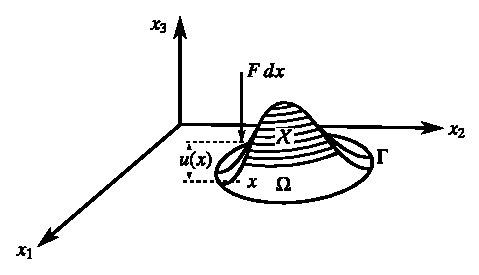
\includegraphics{figure/fig9.1.eps}
\caption{}\label{chap9-fig9.1}
\end{figure}\pageoriginale

The solution $u$ satisfies
\begin{equation*}
J(u)=\min\limits_{v\in K}J(v),\tag{9.2}\label{chap9-eq9.2}
\end{equation*}
where $J(v)=\frac{1}{2}a(v,v)-f(v)$ and is also characterized by the
variational inequalities (cf.\@ Theorem~\ref{chap1-thm1.1}):
\begin{equation*}
a(u,v-u)\geq f(v-u),\quad\text{for all}\quad v\in
K.\tag{9.3}\label{chap9-eq9.3} 
\end{equation*}

We proposed as a problem to show that this problem is interpreted as
the following classical problem (assuming $u\in H^{1}_{0}(\Omega)\cap
H^{2}(\Omega)$). 
\begin{equation*}
\begin{cases}
u\geq \chi\text{~ in~ }\Omega,\\
-\Delta u=f\text{~ where~ }u>\chi,\\
u=0\text{~ on~ }\Gamma.
\end{cases}\tag{9.4}\label{chap9-eq9.4}
\end{equation*}

We have a few regularity results which are listed below:
\begin{itemize}
\item[(i)] If $\Omega$ is convex and $\Gamma$ is a $C^{2}$-boundary
  then $u\in H^{1}_{0}(\Omega)\cap H^{2}(\Omega)$.

\item[(ii)] If $f=0$ and $\Omega$ a convex polygon then also $u\in
  H^{1}_{0}(\Omega)\cap H^{2}(\Omega)$.

\item[(iii)] The norm $||u||_{2,\Omega}$ is bounded above by a
  function of $||f||_{0,\Omega}$ and
  $||\chi||_{2,\Omega}$\pageoriginale in cases (i) and (ii).
\end{itemize}

Our aim in this section is to use the finite element method to
approximate this problem and obtain error estimates. We list our
assumptions now:

Let $\Omega$ be a convex polygon, $f\in L^{2}(\Omega)$, $\chi\in
H^{2}(\Omega)$ and let $u\in H^{2}(\Omega)\cap H^{1}_{0}(\Omega)$.

\begin{remark}\label{chap9-rem9.1}
We cannot assume any more smoothness on $u$ other than
$H^{2}(\Omega)$. For instance in the $1$-dimensional case if $f=0$,
and even if the function is very smooth the points of contact of $u$
with $\chi$ will have discontinuous second derivatives in general;
cf.\@ Fig.~\ref{chap9-fig9.2}.
\begin{figure}[H]
\centering
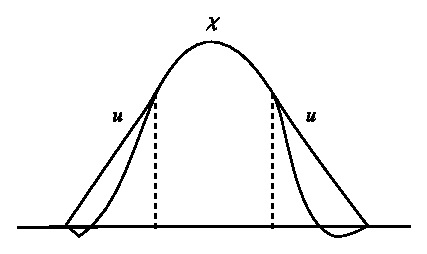
\includegraphics{figure/fig9.2.eps}
\caption{}\label{chap9-fig9.2}
\end{figure}
\end{remark}

With the above assumptions we proceed to the approximate problems,
first in the abstract setting, as usual.

We have the problems $(P_{h})$ associated with the subspaces
$V_{h}\subset V=H^{1}_{0}(\Omega)$. We now choose closed convex
subsets $K_{h}\subset V_{h}$. One has to bear in mind that, in
general, $K_{h}\not\subset K$ (we will see that this is the case in
our approach, sub-sequently).

We find $u_{h}\in K_{h}$ such that for all $v_{h}\in K_{h}$,
\begin{equation*}
a(u_{h},v_{h}-u_{h})\geq f(v_{h}-u_{h}).\tag{9.5}\label{chap9-eq9.5}
\end{equation*}

The existence and uniqueness of the $u_{h}$ follow from
Theorem~\ref{chap1-thm1.1}. 

Let $H$ be a Hilbert space with norm $|\cdot|$ and inner-product
$(\cdot,\cdot)$. Let\pageoriginale $(V,||\cdot||)$ be a subspace such
that $V\hookrightarrow H$, $\overline{V}=H$. Then, as usual, if we
identify $H'$ and $H$, then $H$ will be identified with a subspace of
$V'$. (We will take $V=H^{1}_{0}(\Omega)$ and $H=L^{2}(\Omega)$). Also
as in Sec.~\ref{chap1} (cf.\@ proof of Theorem \ref{chap1-thm1.2}),
for all $u$, $v\in V$ we have
\begin{equation*}
a(u,v)=(Au)(v),\tag{9.6}\label{chap9-eq9.6}
\end{equation*}
where $A:V\to V'$ is a linear map. We now pass on to an abstract error
bound. 

\begin{theorem}[FALK]\label{chap9-thm9.1}
Assume that $f\in H$, $Au\in H$. Then there exists a constant $C$,
independent of $V_{h}$ and $K_{h}$, such that
\begin{equation*}
||u-u_{h}||\leq C\left[\inf\limits_{v_{h}\in
    K_{h}}(||u-v_{h}||^{2}+|u-v_{h}|)+\inf\limits_{v\in
    K}|u_{h}-v|\right]^{\frac{1}{2}}.\tag{9.7}\label{chap9-eq9.7} 
\end{equation*}
\end{theorem}

\noindent
({\em Note:}~The condition $Au\in H=L^{2}(\Omega)$ is satisfied if
$u\in H^{2}(\Omega)$ since $Au=-\Delta u\in L^{2}(\Omega).$)

\begin{proof}
Let $\alpha$ stand for the $V_{h}$-ellipticity constant. Then
\begin{align*}
\alpha || u- u_{h}||^{2} &\leq a(u-u_{h},u-u_{h})\\
&=a(u,u)+a(u_{h},u_{h})-a(u,u_{h})-a(u_{h},u).\tag{9.8}\label{chap9-eq9.8} 
\end{align*}

For any $v\in K$ and any $v_{h}\in K_{h}$, by \eqref{chap9-eq9.3} and
\eqref{chap9-eq9.5}, we have
\begin{equation*}
\begin{cases}
a(u,u)\leq a(u,v)+f(u-v),\\
a(u_{h},u_{h})\leq a(u_{h},v_{h})+f(u_{h}-v_{h}).
\end{cases}\tag{9.9}\label{chap9-eq9.9} 
\end{equation*}

Substituting in \eqref{chap9-eq9.8} we get
\begin{align*}
\alpha ||u-u_{h}||^{2} &\leq
a(u,v)+f(u-v)+a(u_{h},v_{h})\\
& \hspace{2cm}  + f(u_{h}-v_{n})-a(u,u_{h})-a(u_{h},u)\\ 
&= a(u,v-u_{h})-f(v-u_{h})+a(u,v_{h}-u)-f(v_{h}-u)\\
& \hspace{2cm} +a(u_{h}-u,v_{h}-u)\\
&= (f-Au,u-v_{h})+(f-Au,u_{h}-v)+a(u_{h}-u,v_{h}-u)\\
&\leq |f-Au|~|u-v_{h}|+|f-Au|~|u_{h}-v|+M||u_{h}-u||~||v_{h}-u||.
\end{align*}\pageoriginale

Notice that since
$(\sqrt{\dfrac{\alpha}{M}}||u-u_{h}||-\sqrt{\dfrac{M}{\alpha}}||u-v_{h}||)^{2}\geq
0$, we have
$$
||u-u_{h}||~||u-v_{h}||\leq \frac{1}{2}\left(\frac{\alpha}{M}||u-u_{h}||^{2}+\frac{M}{\alpha}||u-v_{h}||^{2}\right),
$$
and hence
$$
\alpha||u-u_{h}||^{2}\leq
C[|u-v_{h}|+|u_{h}-v|]+\frac{\alpha}{2}||u-u_{h}||^{2}+\frac{M^{2}}{2\alpha}||u-v_{h}||^{2} 
$$

Or,
$$
||u-u_{h}||^{2}\leq C[(|u-v_{h}|+||u-v_{h}||^{2})+|u_{h}-v|].
$$

Varying $v_{h}\in K_{h}$ and $v\in K$ and extracting the square root
after taking the infima we get \eqref{chap9-eq9.7}. This completes the
proof. 
\end{proof}

\begin{remark}\label{chap9-rem9.2}
If we have a linear problem then $f=Au$ gives the solution and we get
the original bound \eqref{chap3-eq3.1}.
\end{remark}

\begin{remark}\label{chap9-rem9.3}
From \eqref{chap9-eq9.8} we see that this estimate holds even if
$a(\cdot,\cdot)$ is not symmetric.
\end{remark}

We now apply this to the specific membrane problem. Maintaining our
assumptions on $\Omega$, let $\mathfrak{t}_{h}$ be a triangulation by
triangles of type (1), and let $V_{h}$ be the corresponding subspace
of $V=H^{1}_{0}(\Omega)$.

\begin{remark}\label{chap9-rem9.4}
{\em It is of no practical use if we go to more sophisticated finite
elements, unlike the linear problem.} Since $u\in H^{2}(\Omega)$ is
the maximum smoothness, we may atmost use our abstract estimate
theorems only on the spaces $P_{1}$.
\end{remark}

One may be tempted to try for $K_{h}$ those $v_{h}$ which are $\geq
\chi$ a.e.\@ in $\Omega$. However this is not of value from {\em
  numerical and computational points of view} for\pageoriginale we do
not easily know where exactly our piecewise linear solution functions
would touch $\chi$. We set instead
\begin{equation*}
K_{h}=\{v_{h}\in V_{h};\text{~ At all nodes~ }b \text{~ of~ }
\mathfrak{t}_{h}, v_{h}(b)\geq \chi(b)\}.\tag{9.10}\label{chap9-eq9.10}
\end{equation*}

\eject


\begin{remark}\label{chap9-rem9.5}
~

\begin{figure}[H]
\centering
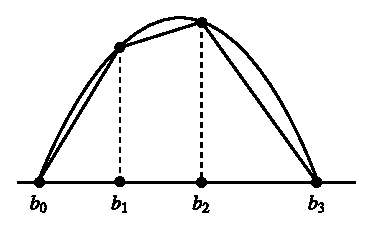
\includegraphics{figure/fig9.3.eps}
\caption{}\label{chap9-fig9.3}
\end{figure}

As seen in Fig.~\ref{chap9-fig9.3}, though for nodes $b$,
$v_{h}(b)\geq \chi (b)$, it does not guarantee that $v_{h}\geq \chi$
a.e. Thus we see that $K_{h}\not\subset K$. Now the relation
\eqref{chap9-eq9.10} is very easy to implement using the computer.
\end{remark}

We now have our main result on the error bound.

\begin{theorem}[FALK]\label{chap9-thm9.2}
There exists a constant $C$ depending on $||f||_{0,\Omega}$ and
$||\chi||_{2,\Omega}$ such that for a regular family of triangulations
$(\mathfrak{t}_{h})$ as above we have
\begin{equation*}
||u-u_{h}||_{1,\Omega}\leq C\ h.\tag{9.11}\label{chap9-eq9.11}
\end{equation*}
\end{theorem}

\begin{remark}\label{chap9-rem9.6}
The order of convergence is therefore the same as that for the linear
problems when we use piecewise linear approximations.
\end{remark}

\begin{proof}
By Theorem~\ref{chap9-thm9.1},
\begin{align*}
||u-u_{h}||_{1,\Omega} &\leq C\left[\inf\limits_{v_{h}\in
    K_{h}}\left(||u-v_{h}||^{2}_{1,\Omega}+|u-v_{h}|_{0,\Omega}\right)+\inf\limits_{v\in K}|u_{h}-v|_{0,\Omega}\right]^{\frac{1}{2}}.
\end{align*}

\begin{itemize}
\item[(i)] We\pageoriginale first estimate the infimum over
  $K_{h}$. Note that if $v_{h}=\pi_{h}u$, then $v_{h}\in V_{h}$. Also
  for all nodes $b$, $v_{h}(b)=\pi_{h}u(b)=u(b)\geq \chi (b)$. Thus
  $v_{h}\in K_{h}$ as well. Thus,
\begin{align*}
\inf\limits_{v_{h}\in
  K_{h}}\left(||u-v_{h}||^{2}_{1,\Omega}+|u-v_{h}|_{0,\Omega}\right)
&\leq ||u-\pi_{h}u||^{2}_{1,\Omega}+|u-\pi_{h}u|_{0,\Omega}\\
&\leq C\ h^{2}\left(|u|^{2}_{2,\Omega}+|u|_{2,\Omega}\right).
\end{align*}

\item[(ii)] For the infimum over $K$, consider $v_{1}=\max
  (u_{h},\chi)$. Clearly $v_{1}\geq \chi$ and $v$ belongs to
  $H^{1}(\Omega)$ because $u_{h}$ and $\chi$ also belong to
  $H^{1}(\Omega)$ (this is a non-trivial result which we assume
  here). Hence $v_{1}\in K$, and thus,
$$
\inf\limits_{v\in K}|u_{h}-v|_{0,\Omega}\leq |u_{h}-v_{1}|_{0,\Omega}.
$$

We have
$$
|u_{h}-v_{1}|^{2}_{0,\Omega}=\int\limits_{\Lambda_{h}}|u_{h}-\chi|^{2}dx,\text{~
  where~ } \Lambda_{h}=\{x;\chi(x)\geq u_{h}(x)\}.
$$
\end{itemize}

If $\pi_{h}\chi$ is the $V_{h}$-interpolate of $\chi$, then for all
nodes $b$, $u_{h}(b)\geq \chi(b)=\pi_{h}\chi(b)$. Since both $u_{h}$
and $\pi_{h}\chi$ are piecewise linear, we may now assert that
$u_{h}\geq \pi_{h}\chi$ everywhere. Thus $u_{h}-\pi_{h}\chi\geq 0$ on
$\Omega$. Thus for all $x\in \Lambda_{h}$, we have
\begin{align*}
0<|(\chi-u_{h})(x)|=(\chi-u_{h})(x) &\leq (\chi-\pi_{h}\chi)(x)\\
&\leq |(\chi-\pi_{h}\chi)(x)|
\end{align*}
and for $x\in \Omega-\Lambda_{h}$, $(\chi-u_{h})(x)=0$, so that
$$
|u_{h}-v_{1}|_{0,\Omega}\leq
\left(\int\limits_{\Omega}|\chi-\pi_{h}\chi|^{2}dx\right)^{\frac{1}{2}}=|\chi-\pi_{h}\chi|_{=0,\Omega}\leq
C\ h^{2}|\chi|_{2,\Omega}. 
$$

Hence
$$
||u-u_{h}||_{1,\Omega}\leq C(h^{2})^{\frac{1}{2}}=Ch,
$$
where\pageoriginale $C$ depends on $|\chi|_{2,\Omega}$ and
$|u|_{2,\Omega}$. However the regularity result (iii) helps us to
bound $|u|_{2,\Omega}$ above by a constant $C$ depending on
$|f|_{0,\Omega}$ and $||\chi||_{2,\Omega}$ which completes the proof
of the theorem.
\end{proof}

\noindent
{\bf References:}~ Two important references are Falk \cite{key11} and
\cite{key12}. For regularity results refer Brezis and Stampacchia
\cite{key3} and Lewy and Stampacchia \cite{key16}. 

Another references is Mosco and Strang \cite{key19}.


